\documentclass{article}
\usepackage{microtype}
\usepackage{graphicx}
\usepackage{booktabs}
\usepackage{hyperref}
\usepackage{xurl}
\newcommand{\theHalgorithm}{\arabic{algorithm}}
\usepackage{icml2026}
\usepackage{amsmath,amssymb,amsthm}
\usepackage[capitalize,noabbrev]{cleveref}
\newtheorem{proposition}{Proposition}
\newcommand{\sig}{\sigma}
\newcommand{\R}{\mathbb R}
\newcommand{\ind}{\mathbf 1}
\newcommand{\HumanMatchMean}{17.82}
\newcommand{\GPTMatchMean}{35.79}
\newcommand{\MatchDiffMean}{17.96}
\newcommand{\MatchDiffLow}{11}
\newcommand{\MatchDiffHigh}{25}
\newcommand{\GPTBootLow}{39.0}
\newcommand{\GPTBootHigh}{82.0}
\newcommand{\MainRuntime}{111.2}
\newcommand{\CrossedPairs}{158}
\newcommand{\TestedPairs}{163}
\newcommand{\CensoredPairs}{5}
\newcommand{\MaxBudgetError}{98}

\icmltitlerunning{Outcome Reversal Audits for Pairwise Leaderboards}
\begin{document}
\twocolumn[
\icmltitle{Outcome Reversal Audits for Pairwise Leaderboards:\\
Exact Balanced Cases and Matched Design Evidence}
\begin{icmlauthorlist}
\icmlauthor{Anonymous Authors}{anon}
\end{icmlauthorlist}
\icmlaffiliation{anon}{Anonymous Institution}
\icmlkeywords{Bradley--Terry, ranking stability, evaluation, sensitivity analysis}
\vskip 0.3in
]
\printAffiliationsAndNotice{}
\begin{abstract}
Pairwise leaderboards summarize heterogeneous comparison designs with a common ranked list, but a small fraction of changed outcomes need not represent a comparable perturbation across designs.
We audit fixed-schedule outcome reversals in public crowdsourced, expert, model-judge, and basketball data, combining influence-guided selection with full Bradley--Terry refits and random-corruption controls.
An elementary balance condition yields an exact minimum reversal budget, providing a reference case for approximate audits and enabling identical-schedule comparisons of human and GPT-4 judgments.
The observed top-two reversal budgets range from one record in Arena to 61 in full MT-Bench GPT-4 data; the latter is certified exact, while the unbalanced-data budgets are feasible witnesses.
Across 500 matched balanced panels, the mean exact budget for reversing GPT-4 versus Claude is \HumanMatchMean{} human judgments versus \GPTMatchMean{} GPT-4 judgments, although this conditional difference does not establish a causal effect of judge type.
Random flips, cluster resampling, alternative challengers, and tie policies expose different failure modes, supporting audits that report the comparison design, uncertainty, and edit unit alongside a percentage.
\end{abstract}

\section{Introduction}
Pairwise evaluation asks which of two participants performed better and aggregates the answers into scores. Its appeal spans crowdsourced model evaluation, expert benchmarks, automated judging, and sports. A ranking, however, compresses several quantities: the fitted score margin, the comparison schedule, the available outcomes, and the uncertainty from observing a particular sample. Two adjacent ranks can be nearly indistinguishable or widely separated. A percentage of all recorded comparisons does not reveal which case applies.

We study an explicit counterfactual: keep the participants and observed pairings fixed, and reverse the outcomes of a small number of decisive records. This represents a sensitivity analysis of recorded labels, whether errors are accidental or selected deliberately. It does not assume the ability to submit votes to a live platform, alter prompts, or change a real sporting result. For basketball the intervention is on the historical results table, not an operational threat model.

Three questions guide the study. How different are selected reversals and uniformly random reversals of the same size? How much of an apparent cross-design contrast survives matching the evaluated model pairs and questions? When can a computed edit budget be interpreted as an exact robustness radius, rather than a successful perturbation found by a heuristic?

Our contribution is a controlled audit of these questions, rather than a new general influence-function algorithm. First, we specialize the perturbation algebra to outcome reversals, whose objective changes by an exactly linear term. We state and prove a balanced-schedule condition under which score ordering equals total-win ordering, so a discrete minimum budget is available without a first-order approximation. Second, we use the public MT-Bench data to build paired human/GPT-4 panels with identical, balanced comparison schedules. Third, we place these results beside public Arena and two NBA seasons, reporting random corruption, cluster uncertainty, alternative challengers, baseline selection rules, and tie-policy sensitivity.

The empirical contrasts resist a single claim that leaderboards are either stable or unstable. Arena's one-record reversal concerns a near-zero margin whose bootstrap interval includes zero. MT-Bench's larger budgets coexist with no observed leader loss at the tested random corruption budgets. In NBA 2015 the runner-up is not the cheapest tested challenger. Even the denominator changes the interpretation: the fraction of all games can be small while the fraction relative to comparisons involving the two focal participants is appreciable. These distinctions matter when interpreting a robustness claim as evidence about model quality or evaluation design.

\section{Related Work}
\citet{chiang2024} describe Arena, the use of pairwise models, and uncertainty in preference-based rankings. \citet{zheng2023} introduce MT-Bench and compare expert and model judgments, including limitations of model judges. Our common score model facilitates a sensitivity comparison; it does not reconstruct every official leaderboard adjustment or equate human preference with sporting strength.

Influence functions approximate how fitted quantities change under data perturbations \citep{koh2017}. \citet{broderick2020} use this approach to assess sensitivity to dropping a small fraction of observations, stressing that conventional uncertainty and worst-case sensitivity answer different questions. We use the same general differentiation principle, but the intervention changes outcomes at fixed sample size and fixed pair counts.

The closest supplied ranking study, \citet{huang2025}, evaluates deletion sensitivity of Bradley--Terry rankings, including Arena and MT-Bench and human/model judgments. We do not claim that influential comparisons or cross-platform sensitivity are new discoveries. Our distinct evidence concerns fixed-schedule reversals, an exact balanced reference case, and paired panels that remove differences in comparison counts and selected question cells. Deletion changes the schedule and can destroy the balance property on which our exact result depends; its budgets cannot be numerically compared to reversal budgets as if the edit units were interchangeable.

\citet{min2025} study vote rigging through new votes and show that comparisons not involving a target can affect its ranking. Our full influence rule likewise permits indirect effects, but here the recorded comparisons are fixed. In our five main top-two audits, endpoint-restricted selection matches unrestricted selection. Thus the availability of indirect effects does not imply a benefit from exploiting them in every dataset. We do not make a priority claim for the familiar balanced-design ordering property; the exact-budget construction is used as an interpretable diagnostic and experimental control.

\section{Audit Definition and Methods}
\subsection{Model, ties, and edit units}
For record $r$, let $a_r,b_r$ be its participants, $x_r=e_{a_r}-e_{b_r}$, and $y_r\in\{0,\tfrac12,1\}$ its outcome for $a_r$. With $\sig(z)=(1+e^{-z})^{-1}$, fit
\begin{equation}\label{eq:loss}
 \hat\theta=\arg\min_{\theta:\,\ind^\top\theta=0}
 \sum_{r=1}^N\left[\log(1+e^{x_r^\top\theta})-y_rx_r^\top\theta\right]
 +\frac{\lambda}{2}\|\theta\|_2^2.
\end{equation}
We use natural log-odds scores and $\lambda=10^{-3}$ on the \emph{summed} loss. The small common ridge ensures unique finite estimates, including in resamples. It is not scaled by $N$. We test other penalty strengths. A tie contributes a half-win cross-entropy term; this is a specified working score model, not a generative model of ties.

A permitted edit sends $y_r$ to $1-y_r$ for a decisive record, at unit cost. Ties are held fixed. A record may be reversed at most once, and pair identities are unchanged. GPT-4 records already aggregate the dataset's judging procedure; a unit is one released judgment, not necessarily one underlying API call. For a chosen set $S$, $|S|$ is the cost. We report both $|S|/N$ and $|S|/E_{ij}$, where $E_{ij}$ counts records involving either focal participant, counting their direct matches once. The latter is an exposure normalization, not necessarily the fraction of those records actually edited: unrestricted selection may also use other participants. Counts and fractions relative to decisive records are supplied in the artifacts.

For a fixed original leader $i$ and challenger $j$, let $g_{ij}=\hat\theta_i-\hat\theta_j>0$. The exact pair radius is
\begin{equation}\label{eq:radius}
 K^*_{ij}=\min_S\{|S|:\hat\theta_i^{(S)}<\hat\theta_j^{(S)}\}.
\end{equation}
Equality is not a strict reversal. The exact leader-loss radius is $\min_{j\ne i}K^*_{ij}$. These two targets must be distinguished: the original runner-up need not be the least costly challenger. A successful heuristic set yields an \emph{upper bound} on this minimum. Failure to find a set is not a stability certificate.

\subsection{Linear selection with full refitting}
Reversals have a useful exact identity. Define $b_S=\sum_{r\in S}(1-2y_r)x_r$. The perturbed objective is
\begin{equation}\label{eq:linearperturb}
 L_S(\theta)=L(\theta)-b_S^\top\theta.
\end{equation}
Its Hessian as a function of $\theta$ is unchanged, although its value at the new optimum can differ. Let $H$ be the Hessian of \cref{eq:loss} at $\hat\theta$, restricted to centered vectors, and $c=e_i-e_j$. Then
\begin{equation}\label{eq:influence}
 \hat\theta^{(S)}-\hat\theta\simeq H^{-1}b_S,\qquad
 g_{ij}^{(S)}\simeq g_{ij}-\sum_{r\in S}h_r,
\end{equation}
where $h_r=-(1-2y_r)c^\top H^{-1}x_r$. Sorting positive $h_r$ in decreasing order exactly solves the linearized cardinality problem. The first cumulative sum strictly exceeding $g_{ij}$ defines $K_{\rm lin}$; it is neither an exact radius nor a certificate.

We fix this ordering at the initial fit and refit after \emph{each} prefix until the first strict reversal. We denote the observed prefix length by $K_{ij}$ and retain the before/after gaps and selected row indices. We do not assume monotonicity to perform a binary search. Fits aggregate comparisons by unordered pair and use damped Newton steps. The numerical crossing tolerance is $10^{-9}$; convergence requires maximum gradient magnitude below $10^{-8}$.

Baselines use the same refitting procedure: restrict positive influence to records involving either endpoint; restrict it to direct head-to-head records; or rank by the reduction in total-win margin, independent of the Hessian. Ties in selection scores follow input row order. A random-corruption control samples $k$ distinct decisive rows uniformly and refits. It measures typical behavior under a specified corruption distribution, not worst-case behavior.

\subsection{An exact reference case}
Let $n_{uv}$ be the number of comparisons of participants $u,v$, and $W_u$ the total fractional wins of $u$, including half-wins for ties.
\begin{proposition}[Pair balance]\label{prop:balance}
Suppose $n_{ik}=n_{jk}$ for every $k\notin\{i,j\}$, and use a common $\lambda>0$ in \cref{eq:loss}. Then
\[
 \operatorname{sign}(\hat\theta_i-\hat\theta_j)
 =\operatorname{sign}(W_i-W_j).
\]
This remains true after any allowed outcome reversals. Let $v_r$ be the reduction of $W_i-W_j$ from reversing decisive record $r$, and order the positive reductions as $v_{(1)}\ge v_{(2)}\ge\cdots$. For $W_i>W_j$,
\begin{equation}\label{eq:exact}
 K^*_{ij}=\min\left\{k:\sum_{\ell=1}^k v_{(\ell)}>W_i-W_j\right\},
\end{equation}
with value $\infty$ if no such $k$ exists.
\end{proposition}
The positive reductions are two for reversing a win of $i$ against $j$, and one for reversing a win of $i$ against a third participant or a loss of $j$ against one. The proof subtracts the two score equations: every term has the sign of $\theta_i-\theta_j$ under pair balance. Outcomes do not enter the counts, so reversals preserve the condition. Sorting the discrete reductions both constructs a successful set and proves that fewer edits cannot suffice; \cref{app:proof} gives details.

A complete schedule with the same count for every pair satisfies pair balance for all participants. Hence minimizing \cref{eq:exact} over challengers gives an exact leader-loss radius. This does not extend automatically to sparse or imbalanced schedules, nor to deleting ties. It also explains why small random error can behave differently: in a balanced schedule, uniform reversal of $k$ out of $D$ decisive rows gives
\begin{equation}\label{eq:expect}
 \mathbb E[W_i^{(S)}-W_j^{(S)}]
 =\left(1-\frac{2k}{D}\right)(W_i-W_j).
\end{equation}
For $k<D/2$ the expected win-margin sign persists. This is an expectation identity, not a bound on the probability of a rank reversal.

\section{Data and Experimental Design}
\begin{table*}[t]
\caption{Fixed snapshots and original top-two score gaps. Intervals are percentile intervals from 1,000 cluster bootstrap refits of the \emph{fixed original pair}; ``Top kept'' is the resampling frequency of retaining the original leader. Cluster definitions differ across datasets and do not eliminate all dependence.}
\label{tab:data}
\centering\small\begin{tabular}{lrrrrrrr}
\toprule
Data & $N$ & $M$ & Tie \% & Clusters & Gap & 95\% interval & Top kept \% \\
\midrule
Arena & 57,477 & 64 & 30.9 & 51734 & 0.004 & [-0.100, 0.097] & 52.8 \\
MT human & 3,355 & 6 & 23.2 & 80 & 0.378 & [0.110, 0.638] & 99.7 \\
MT GPT-4 & 2,400 & 6 & 25.0 & 80 & 0.821 & [0.540, 1.120] & 100.0 \\
NBA 2014 & 1,230 & 30 & 0.0 & 163 & 0.204 & [-0.451, 0.975] & 58.8 \\
NBA 2015 & 1,230 & 30 & 0.0 & 162 & 0.621 & [-0.229, 1.562] & 87.9 \\
\bottomrule
\end{tabular}

\end{table*}

\paragraph{Public data.}
We use the 57,477-record Arena human-preference snapshot, both released MT-Bench splits, and the 2014 and 2015 NBA regular seasons from FiveThirtyEight's historical results \citep{nba}. Dataset commits, file hashes, selection code, and licenses are recorded in the reproducibility package. All source files matched the specified SHA-256 values. We use all Arena participants and records, with no score- or exposure-based inclusion threshold. MT-Bench has six participants and 80 questions; its human split includes expert and author annotators. Each GPT-4 pair has 160 records, making the full schedule balanced. Its 380 ``tie (inconsistent)'' records are treated as half-wins within the 600 total ties. Sensitivity checks omit them and, separately, omit all ties.

For NBA we retain the NBA league, non-playoff games, the two stated season years, and $\texttt{\_iscopy}=0$, obtaining one row per game. We do not use Elo scores, point margins, or forecasts. Each season has 30 teams, rather than pooling franchises across eras. This keeps participants and the season window interpretable. The model omits home advantage and changing team strength, so its ranking is a static aggregate, not a reconstruction of official standings or a sports prediction system.

\paragraph{Primary targets and budgets.}
The primary audit compares the original first and second ranks. The pairs are GPT-4-1106-preview versus GPT-4-0125-preview in Arena, GPT-4 versus Claude-v1 in both MT-Bench splits, San Antonio versus Oklahoma City in NBA 2014, and Golden State versus Atlanta in NBA 2015. We additionally audit every challenger to the original leader and all adjacent pairs within the original top ten (all participants for MT-Bench): \TestedPairs{} distinct pair problems. Main top-pair searches permit up to 20\% of records, and broader searches up to 5\%; all observed primary crossings occur below 5\%. A missing crossing is recorded as censored.

Random corruption uses 500 independent subsets at each rounded-up budget in $\{0.05,0.1,0.2,0.5,1,2,5\}\%$ of all records, plus the observed primary crossing budget. Duplicate integer budgets are merged. We record original-leader loss, original-pair reversal, and Kendall's $\tau$ over all fitted scores. Wilson intervals describe Monte Carlo uncertainty of loss probabilities. This random design selects from decisive rows, while its x-axis counts edits relative to all rows; the distinction matters when tie rates differ.

\paragraph{Resampling uncertainty.}
We draw 1,000 cluster bootstrap samples per dataset, using whole MT-Bench questions, exact Arena prompt-string hashes, and NBA calendar dates as clusters. The clusters are sampled with replacement, retaining all records in each sampled cluster. Intervals describe the original named pair without reselecting it in each resample. They do not adjust for selecting the original winner and are not simultaneous rank confidence sets. User/session identifiers are unavailable in the Arena CSV, and identical text does not capture all shared-user dependence. NBA date clustering also does not capture dependence across a team's season. We therefore use these intervals as conditional uncertainty diagnostics, not population-level guarantees.

\paragraph{Matched schedules.}
To compare the two MT-Bench judgment designs, a cell is an unordered model pair, question, and turn. There are 1,814 cells observed by both designs. The minimum shared-cell count over the 15 pairs is 99. For each of 500 panels, we uniformly select 99 shared cells without replacement \emph{within each pair}, then choose one available human judgment per selected cell uniformly; GPT-4 supplies its unique corresponding record. Both panels thus contain 1,485 records with exactly the same pair/question/turn schedule and 99 records per pair. Human annotators are not forced to match across cells. The balance proposition gives exact pair and leader radii for both panels.

We fix GPT-4 versus Claude-v1 as the paired contrast across panels, and also report the minimum over all challengers. Panel quantiles summarize variation from this subsampling and annotator selection procedure; they are \emph{not} population confidence intervals. Questions, response pairs, and the available human annotations remain those of the original dataset. Matching removes measured schedule differences, not possible selection bias or judge self-preference.

\paragraph{Implementation and checks.}
All numerical experiments use CPU double precision and a recorded base seed, 20261028, with deterministic offsets for separate procedures. The main experiment took \MainRuntime{} seconds with single-threaded numerical libraries on an Intel Xeon Gold 6230 host. We checked the optimizer against independent BFGS optimization, the derivative against finite differences, and the balanced formula against exhaustive subset enumeration on a small synthetic \emph{unit test}. No synthetic data are used as empirical evidence. We numerically checked both sides of every exact full-GPT pair threshold and all matched-panel focal thresholds. Code and generated tables are included.

\section{Results}
\begin{table*}[t]
\caption{Reversal budgets and matched-budget random corruption. $K_{12}$ is the first fully refitted prefix reversing the original top pair; $K_{\rm lead}$ is the smallest found budget across challengers. These are feasible upper bounds on unbalanced data. For full MT GPT-4, both displayed refitted budgets equal the exact optimum. Random loss uses $k=K_{12}$, with 95\% Wilson intervals from 500 runs. A zero observed rate is not zero probability.}
\label{tab:radii}
\centering\small\begin{tabular}{lrrrrrr}
\toprule
Data & $K_{\rm lin}$ & $K_{12}$ & $100K_{12}/N$ & $100K_{12}/E_{12}$ & $K_{\rm lead}$ & Random top loss \% \\
\midrule
Arena & 1 & 1 & 0.0017 & 0.01 & 1 & 0.8 [0.3, 2.0] \\
MT human & 45 & 46 & 1.3711 & 2.52 & 46 & 0.0 [0.0, 0.8] \\
MT GPT-4 & 56 & 61 & 2.5417 & 4.24 & 61 & 0.0 [0.0, 0.8] \\
NBA 2014 & 4 & 4 & 0.3252 & 2.50 & 4 & 0.0 [0.0, 0.8] \\
NBA 2015 & 7 & 8 & 0.6504 & 4.94 & 7 & 0.0 [0.0, 0.8] \\
\bottomrule
\end{tabular}

\end{table*}

\subsection{A small fraction has several meanings}
\Cref{tab:radii} shows substantial variation in the selected top-pair budgets: one Arena record, 46 MT human records, 61 MT GPT-4 records, and four or eight NBA games. These are changes to the analyzed frozen tables, not assertions of past manipulation. For Arena the result is also a trivial exact minimum for the fitted pair: zero edits retain its strict initial order, and one edit reverses it. For other unbalanced cases, we do not establish optimality.

Exposure normalization changes the scale of the comparison. NBA 2014 requires 0.3252\% of all season games but 2.50\% relative to the two teams' comparison exposure; the MT human values are 1.3711\% and 2.52\%, respectively. Their global fractions differ appreciably, while their exposure fractions nearly coincide. This does not make the designs equivalent: opponents, outcome margins, and dependence remain different. It does show why a global percentage alone can exaggerate a contrast. Arena remains a particularly small-budget case under either denominator.

The small Arena budget also needs its uncertainty context. Its original gap is approximately 0.004 log-odds, with a bootstrap interval spanning zero and only 52.8\% retention of the original leader. The two MT-Bench gaps have positive bootstrap intervals in our resampling procedure. Both NBA intervals span zero despite their differing point margins and edit budgets. These diagnostics reinforce that a change in displayed rank can concern an uncertain distinction rather than a large change in assessed performance.

\subsection{Selected edits and random errors diverge}
\begin{figure*}[t]
\centering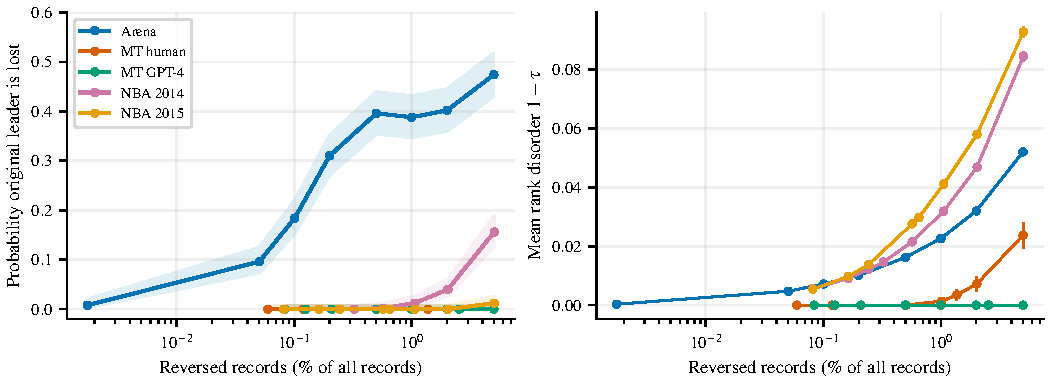
\includegraphics[width=\textwidth]{../figures/noise.pdf}
\caption{Uniform random outcome reversals, with 500 refits per point. Left: probability that the original leader is no longer first; shading gives 95\% Wilson intervals. Right: whole-ranking disorder; bars are 1.96 Monte Carlo standard errors of the mean. Percentages use all records, although only decisive records are eligible. The first point or extra point can be a dataset's targeted crossing budget.}
\label{fig:noise}
\end{figure*}
At the selected top-pair budget, the observed random leader-loss rate is 0.8\% for Arena and zero in each other dataset, with a Wilson upper endpoint of approximately 0.8\% for each zero count (\cref{tab:radii}). Thus selected and uniform perturbations should not be summarized by the same qualitative word ``sensitive.'' In particular, a worst-case witness is not evidence that random mistakes of that count typically change the winner.

At 5\% of all records, original-leader loss under random corruption occurs in 47.4\% of Arena runs, 15.6\% of NBA 2014 runs, and 1.2\% of NBA 2015 runs; neither MT-Bench split loses its leader in the 500 runs. Whole-ranking changes nevertheless occur. At this budget, mean Kendall correlation is about 0.948 for Arena and 0.907 for NBA 2015. Hence the dataset with a more stable leader can have more movement elsewhere in its ranking. \Cref{fig:noise} reports the complete budget curves and Monte Carlo uncertainty, rather than selecting only these endpoints.

\subsection{The easiest challenger can be third}
For NBA 2015, seven selected reversals put Houston, originally third, above Golden State, while eight are needed along the chosen path for Atlanta, originally second. This is a strictly better \emph{found witness}, not a proof that seven is globally minimal. In all other primary datasets the smallest found leader-loss budget coincides with the top-pair budget.

The direct-head-to-head baseline fails to reverse either NBA primary pair using its available helpful outcomes: San Antonio has no recorded win over Oklahoma City in these season records, while the available Golden State win over Atlanta is insufficient. Endpoint-restricted, unrestricted influence, and raw-win-gain rules all achieve the same primary crossing counts (\cref{tab:baselines}). This is a useful negative result: the more general selection rule offers no count advantage on these five main pairs. Neither the existence of graph-mediated influence nor the algorithm's sophistication substitutes for checking the actual schedule and outcome supply.

\subsection{Balanced matching preserves a judge contrast}
The full GPT-4 split has an exact focal and leader-loss radius of 61, certified by \cref{prop:balance}. Its total-win margin between GPT-4 and Claude-v1 is 121; 60 helpful direct reversals leave a positive margin, and 61 reverse it. A question-cluster bootstrap that preserves this complete schedule gives a percentile interval of [\GPTBootLow{}, \GPTBootHigh{}] for the focal radius, showing that an exact radius on the observed table can still vary under resampling.

\begin{figure*}[t]
\centering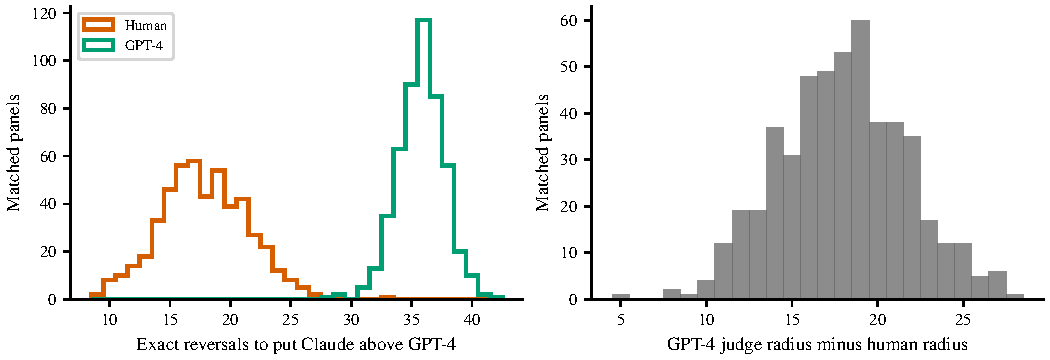
\includegraphics[width=\textwidth]{../figures/matched.pdf}
\caption{Exact focal radii on 500 paired, balanced MT-Bench schedules (1,485 judgments each). Left: human and GPT-4 distributions for making Claude-v1 strictly exceed GPT-4. Right: within-panel differences. These repeated-panel distributions quantify subsampling and annotation-selection variability conditional on the released data; they are not independent new benchmark replications.}
\label{fig:matched}
\end{figure*}

In the matched panels, the mean exact GPT-4-versus-Claude radius is \HumanMatchMean{} for human judgments and \GPTMatchMean{} for GPT-4 judgments. The paired mean difference is \MatchDiffMean{} records; its central 95\% panel interval is [\MatchDiffLow{}, \MatchDiffHigh{}]. Every sampled paired difference is positive. Because the two panels have identical participants, cells, and total sizes, the direction of this contrast cannot be attributed solely to those schedule differences. Under balance it is directly accounted for by different total-win margins and available favorable outcomes, rather than by an influence approximation.

This is not evidence that automated judging is generally more reliable. A larger margin can reflect stronger consensus, a judge's systematic preferences, or bias. GPT-4 is both judge and a competing model here, a concern consistent with the self-enhancement limitations discussed by \citet{zheng2023}. The matched design does not separate these explanations. It identifies an outcome-level contrast for the released response pairs, conditional on their selection. Moreover, the focal radius and the full leader radius sometimes differ in human panels; both summaries are reported in \cref{tab:matched}.

\subsection{Approximation and policy choices matter}
Linear prediction is close at some primary thresholds but is not uniformly exact: it predicts 56 edits rather than the certified 61 in full GPT-4 data and seven rather than eight for the NBA 2015 top pair. Among \TestedPairs{} broader pair problems, \CrossedPairs{} cross within the allowed searches; the remaining \CensoredPairs{} are censored. Among the crossed cases, absolute threshold error reaches \MaxBudgetError{} records. Per-dataset median relative errors range from about 3\% to 23\% (\cref{tab:approx}). These are correlated audits within five datasets, not independent evidence for a universal error distribution. Approximation is useful for selecting records, but reporting its predicted crossing as a measured reversal would misstate results.

Tie handling has a larger qualitative effect than numerical precision. Dropping all Arena ties reverses its original top pair before any further edit; thus its original one-record finding is conditional on the tie policy. Omitting all ties changes the MT human and GPT-4 thresholds for their original pairs to 42 and 39, respectively. Omitting only GPT-4's inconsistent ties gives 47. Those omissions change pair counts, so the balanced optimum for the full dataset no longer applies. The global percentage ordering of the full MT splits persists in these particular omission checks, but the raw count ordering does not persist when all ties are omitted.

Changing $\lambda$ from the default to $10^{-5}$ or $0.1$ leaves all five main counts unchanged; $\lambda=1$ increases the Arena count to two and leaves the other counts unchanged. Restricting MT humans to expert-labeled annotators gives 41 edits on 2,668 records; removing the one repeated annotation key leaves the primary threshold at 46. Complete ablation results appear in \cref{app:more}. These checks support some local robustness of the comparisons while also identifying a concrete failure of tie-policy invariance.

\section{Discussion and Limitations}
This study supports reporting a \emph{profile} of stability: the edit operation and eligible rows, a focal pair or leader-loss target, the observed gap, the comparison exposure, random-corruption behavior, and refitted witnesses. An uncertainty interval and a selected-edit budget should accompany each other because neither implies the other. The balanced case is particularly transparent: exact robustness is a property of the observed win margin and available reversal gains, not a claim about a judge's truthfulness.

Several restrictions limit generalization. We analyze frozen historical snapshots; model names and the live ranking can change. We use one common, static, scalar BT score model. Position effects, home advantage, task-specific skill, nontransitive preferences, and time trends are not modeled. Ties are represented as half-wins, and changing that decision materially affects some results. Ridge strength is tested, but we do not compare alternative ranking model families. No conclusion here establishes that BT is the best ranking rule.

The adversarial budget assumes arbitrary access to eligible recorded outcomes, uniform edit cost, and knowledge of the released table. Actual annotation mistakes may be structured, while a real adversary may face identification, access, or authentication constraints. Corrupting a released GPT-4 judgment is not economically equivalent to corrupting one human vote or an NBA result. Exposure fractions improve interpretability but do not make such costs exchangeable. We also do not audit deletion or new-vote injection, whose effects and costs differ.

Matching controls observed cells but cannot randomize judge identity or recover missing human annotations. Panel variation and bootstrap intervals are conditional on the source questions and measurement process; the human annotator, user, and team dependence structures are not fully observed or resampled. Results on these benchmarks therefore cannot rank entire evaluation-design classes by reliability. Unbalanced-data attacks remain heuristic upper bounds except for the trivial one-edit optimum, and censored searches provide no lower bound. The exact balanced result is a reference case, not a solution to arbitrary discrete perturbation optimization.

A practical conclusion follows within these limits: before treating a small edit percentage as evidence of a defective leaderboard, inspect the underlying gap and exposure, specify the edit unit, verify the claimed crossing by refitting, and check alternatives to the original runner-up. Before attributing a cross-dataset contrast to judge quality, match the comparison design where possible and retain the uncertainty about bias and sampling that matching cannot remove.

\clearpage
\section*{Impact Statement}
This work studies the reliability of aggregate rankings and provides reproducible sensitivity diagnostics. It can help evaluation providers avoid overstating small differences and prioritize data review. The same diagnostics could identify influential records for misuse. Our experiments are offline modifications of public historical data; no votes were submitted, no users were contacted, and no live leaderboard was altered. We release analysis code and derived numerical results, without redistributing raw conversation text. We make no claim that particular participants or annotators manipulated data. Sports examples concern recorded-result sensitivity, not actionable interference with games.

\section*{Use of AI Assistance}
An OpenAI Codex assistant autonomously designed the study, wrote and executed the code, read the directly accessed permitted literature, and drafted this manuscript. All reported empirical results come from the accompanying executed CPU code; no LLM API was used to create new judgments. Numerical verification is documented, but there was no independent human scientific review. This disclosure describes research assistance and does not designate an AI system as an author.

\bibliography{references}
\bibliographystyle{icml2026}

\clearpage
\appendix
\onecolumn
\section{Proofs and Exactness Conditions}\label{app:proof}
Let $n_{uv}=n_{vu}$, $n_{uu}=0$, and $d_u=\sum_{v\ne u}n_{uv}$. With fractional outcomes the gradient of the summed objective is
\[
 \frac{\partial L}{\partial\theta_u}
 =\sum_{v\ne u} n_{uv}\sig(\theta_u-\theta_v)-W_u+\lambda\theta_u.
\]
For a centered optimum, the Lagrange multiplier for the centering constraint is zero because the sum of gradients is $\lambda\sum_u\theta_u=0$. The common ridge makes the objective strictly convex. Subtracting the score equations for $i$ and $j$ under the pair-balance condition gives
\begin{align*}
 W_i-W_j
 &=n_{ij}\{2\sig(\theta_i-\theta_j)-1\}\\
 &\quad+\sum_{k\notin\{i,j\}}n_{ik}\{\sig(\theta_i-\theta_k)-\sig(\theta_j-\theta_k)\}
 +\lambda(\theta_i-\theta_j).
\end{align*}
Since the sigmoid is strictly increasing, every nonzero term has the sign of $\theta_i-\theta_j$, and the ridge term makes the sign strict when the difference is nonzero. At equality all terms are zero. This proves the ordering identity, including equality, and does not require the data-generating BT model to be correct. Pair balance also implies $d_i=d_j$.

Reversing an outcome changes only $W$, not $n$. For a decisive row with canonical endpoints $a_r,b_r$, its decrease in the focal win margin is
\[
 v_r=(2y_r-1)\{\ind[a_r=i]-\ind[a_r=j]-\ind[b_r=i]+\ind[b_r=j]\}.
\]
Its possible positive values are one and two. A record outside the focal endpoints has zero gain. Because the win margin is linear in outcomes, after reversing any $k$ rows its reduction cannot exceed the sum of the $k$ largest positive $v_r$. If that sum is at most the original margin, no $k$-edit set strictly reverses the score order. When the sum exceeds the margin, choosing those rows achieves a reversal. This proves \cref{eq:exact}, with the important strict inequality handling integer and half-integer margins. If gains are exhausted before crossing, the permitted intervention cannot cause the pair reversal.

For a balanced complete graph, every challenger satisfies the premise. The original leader loses its unique lead exactly when some other participant strictly exceeds it. Taking the minimum of the exact pair radii therefore gives the exact leader-loss radius. The proof does not imply that the runner-up minimizes this quantity, even under balance, because the supply of two-unit and one-unit gains can differ.

For \cref{eq:expect}, write $W_i-W_j=(d_i-d_j)/2+\sum_r(y_r-1/2)c^\top x_r$. Balance makes the degree term zero; tie terms vanish. Every decisive record is included in a uniform size-$k$ subset with marginal probability $k/D$, so every centered outcome has expectation multiplied by $1-2k/D$. Linearity of expectation proves the identity without independent inclusion indicators. It does not imply $\mathbb E[\hat\theta^{(S)}]$ has the analogous scaling, because fitting is nonlinear.

The linear influence expression follows by differentiating the score equation for $L(\theta)-t b_S^\top\theta$ at $t=0$: $H\dot\theta=b_S$. Centering is respected since $\ind^\top b_S=0$. The implementation adds a constant-direction projector to the Hessian solely for numerical stability; it does not change a centered solution. A finite edit can move to a region with different Hessian values despite the exact identity of the Hessian \emph{functions} in \cref{eq:linearperturb}. Hence the linear cumulative threshold has no exactness guarantee merely because label changes leave the design fixed.

\section{Additional Empirical Results}\label{app:more}
\begin{table}[!ht]
\caption{Primary top-pair baseline budgets from full refits. Dashes mean the direct baseline exhausted available helpful outcomes without crossing; they are not missing experiments. All selected main witnesses involve at least one focal endpoint. The win-gain rule is scored in win units and has no reported logit-linear prediction.}
\label{tab:baselines}\centering\begin{tabular}{lrrrr}
\toprule
Data & Full & Endpoint & Direct & Win gain \\
\midrule
Arena & 1 & 1 & 1 & 1 \\
MT human & 46 & 46 & 46 & 46 \\
MT GPT-4 & 61 & 61 & 61 & 61 \\
NBA 2014 & 4 & 4 & -- & 4 \\
NBA 2015 & 8 & 8 & -- & 8 \\
\bottomrule
\end{tabular}

\end{table}

\begin{table}[!ht]
\caption{Balanced matched-panel summaries. Panel intervals are 2.5th--97.5th percentiles of 500 panel outcomes, not confidence intervals for a population effect. The human original leader is GPT-4 in every panel, while the runner-up is Claude-v1 in 472 panels and GPT-3.5-turbo in 28. The human leader radius differs from the fixed GPT-4/Claude radius in 24 panels.}
\label{tab:matched}\centering\small\begin{tabular}{lrrrrr}
\toprule
Judge & Mean $K_{4,C}$ & Panel interval & Mean $K_{\rm lead}$ & Mean $W_4-W_C$ & Mean gap \\
\midrule
Human & 17.82 & [11.0, 25.0] & 17.72 & 34.41 & 0.298 \\
GPT-4 & 35.79 & [32.0, 39.5] & 35.79 & 70.30 & 0.770 \\
\bottomrule
\end{tabular}

\end{table}

\begin{table}[!ht]
\caption{Approximation error among crossed broader pair audits, comparing the linear predicted threshold with the first fully refitted crossing along the same ordered prefix. Relative error divides absolute count error by the refitted count. Top-pair results are included; each distinct pair occurs once. Uncrossed cases are excluded from error summaries and included in tested denominators.}
\label{tab:approx}\centering\begin{tabular}{lrrrr}
\toprule
Data & Crossed/tested & Median $|\Delta K|$ & Max & Median rel. \% \\
\midrule
Arena & 71/71 & 9.0 & 98 & 3.1 \\
MT human & 7/9 & 3.0 & 26 & 4.4 \\
MT GPT-4 & 6/9 & 4.0 & 16 & 7.3 \\
NBA 2014 & 37/37 & 2.0 & 15 & 14.3 \\
NBA 2015 & 37/37 & 4.0 & 15 & 23.1 \\
\bottomrule
\end{tabular}

\end{table}

\begin{figure}[!ht]
\centering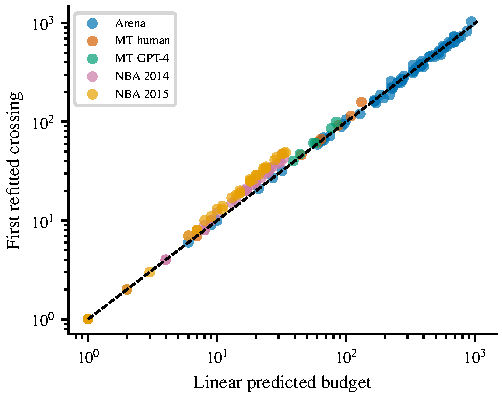
\includegraphics[width=.5\textwidth]{../figures/approximation.pdf}
\caption{Prediction versus refitted crossing for the \CrossedPairs{} crossed pair problems. The dashed line is equality. Five censored problems are not plotted; the figure therefore does not characterize approximation error beyond the tested search budgets.}
\label{fig:approx}
\end{figure}

\clearpage
\begin{table}[t]
\caption{Penalty and tie-policy sensitivity. ``Base'' uses $\lambda=10^{-3}$ with all ties retained; the next columns use the indicated penalty on the summed loss. Ridge variants audit their own top pair, which remains the same in these runs. ``No ties'' removes all half-win records and audits the original named top pair; zero means that pair is already reversed before further edits. NBA has no ties, so its no-tie run repeats the baseline as a consistency check.}
\label{tab:ablation}\centering\begin{tabular}{lrrrrrr}
\toprule
Data & Base & $10^{-5}$ & $0.1$ & $1$ & No ties & No-tie gap \\
\midrule
Arena & 1 & 1 & 1 & 2 & 0 & -0.034 \\
MT human & 46 & 46 & 46 & 46 & 42 & 0.532 \\
MT GPT-4 & 61 & 61 & 61 & 61 & 39 & 1.104 \\
NBA 2014 & 4 & 4 & 4 & 4 & 4 & 0.204 \\
NBA 2015 & 8 & 8 & 8 & 8 & 8 & 0.621 \\
\bottomrule
\end{tabular}

\end{table}

\begin{table}[!ht]
\caption{Additional preprocessing checks. Expert-only removes author-labeled MT annotations; deduplicated key retains the first record for each question/pair/turn/judge key; omission of inconsistent GPT-4 judgments retains consistent ties. These thresholds are refitted witnesses and are not claimed optimal.}
\label{tab:supplement}\centering\begin{tabular}{llrrrr}
\toprule
Data & Variant & $N$ & $K_{12}$ & Gap & $100K_{12}/N$ \\
\midrule
MT human & Experts only & 2668 & 41 & 0.403 & 1.54 \\
MT human & Deduplicated key & 3354 & 46 & 0.378 & 1.37 \\
MT GPT-4 & Omit inconsistent & 2020 & 47 & 0.994 & 2.33 \\
\bottomrule
\end{tabular}

\end{table}

\subsection{Data provenance and preprocessing}
All data are public and were downloaded without credentials. The Arena source is \texttt{lmarena-ai/arena-human-preference-55k}, commit \nolinkurl{18c298340948c0e7f7727399fd459cca6ce0ca6f}, under Apache-2.0. MT-Bench is \texttt{lmsys/mt\_bench\_human\_judgments}, commit \texttt{f7d2896d2cc5d80f8b55c2bbc722613555233c25}, under CC-BY-4.0. NBA is the FiveThirtyEight data repository, commit \texttt{4c1ff5e3aef1816ae04af63218015066e186c147}, also under CC-BY-4.0. The full URL, byte count, and SHA-256 of each source file are recorded in \texttt{data/manifest.json} locally and \texttt{DATA\_MANIFEST.json} in the submission. Raw data are stored under \texttt{data/raw/} and are excluded from the submitted archive.

Canonical preprocessing orders model names lexicographically and changes $y$ to $1-y$ if the endpoints are swapped. The datasets contain no same-participant rows in our selected samples. Arena's three outcome indicators are checked to sum to one and its record identifiers to be unique. Only model identities, outcome flags, identifiers, and prompt hashes are used. Response texts are unused. The MT human main analysis preserves the released 3,355 records, including one repeated annotation key; the extra deduplication run addresses that choice. NBA game identifiers are checked to be unique after filtering.

The balanced matched panels sample from each pair's shared cells, not from all questions as indivisible blocks. Consequently the exact balance property is preserved but the set of questions represented for one pair can differ from that for another. Both judge types still see the same cells within a panel. The separate full-GPT radius bootstrap resamples whole questions; every question contains the complete set of pairs and both turns, so this bootstrap also preserves pair balance. Its 1,000 samples use an independent seed from the gap bootstrap.

\subsection{Interpretation of uncertainty and negative results}
The primary targeted counts are deterministic conditional on the dataset, penalty, selection rule, and row-order tie breaking. They therefore do not need a Monte Carlo confidence interval. Uncertainty about the data sample is instead assessed by the cluster gap bootstrap and, for the complete GPT-4 schedule, the exact-radius bootstrap. The repeated matched panels quantify sensitivity to a specified construction rule. Reporting these intervals as interchangeable would overstate inferential precision.

All successful thresholds are verified with before/after refits. All damped-Newton experiment fits met the stated convergence test. All ten independent real-data BFGS checks returned precision-loss warnings; these checks nevertheless met a separate $10^{-5}$ gradient-residual bound and agreed with the main fits within $10^{-5}$ in scores. The direct NBA baseline failures and the five capped broad searches are retained. We did not attempt exact combinatorial optimization for arbitrary schedules; a better selection rule might improve an unbalanced upper bound. We also did not generate fresh judgments or obtain multiple independent realizations of an evaluation platform. Such unperformed work is not represented by the 500 random-corruption runs or matched panels.

\section{Reproduction Guide and Completed Checklist}\label{app:repro}
The package includes code, locked dependencies, conference styles, generated artifacts, numerical results, and manuscript source/PDF. \texttt{README.md} maps commands to outputs; \texttt{run\_all.sh} reruns the pipeline. The base seed is 20261028. Main random seeds add $100d$ for dataset index $d$ in the order Arena, human MT, GPT-4 MT, NBA 2014, NBA 2015; the gap bootstrap adds a further one. Matched panels use 20270028 and the exact-radius bootstrap 20273028. Unit tests use seed 174.

Python 3.11, NumPy 2.4.6, SciPy 1.17.1, pandas 3.1.0, PyArrow 26.0.0, and Matplotlib 3.11.2 were used; exact dependencies are locked. Numerical libraries use one thread. Main, matched-panel, and supplemental runs took \MainRuntime{}, about 17, and about 11 seconds respectively. These measured times exclude setup and are hardware-dependent.

\paragraph{Conference format.}
This manuscript uses the unmodified official ICML 2026 submission style. Official instructions allow eight main pages, excluding references, impact, and appendices. No in-paper checklist is supplied in the consulted official materials; this completed checklist is voluntary. A separate plain-language summary is included; no submission or acceptance is claimed.

\begin{enumerate}
\item \textbf{Claims and scope: Yes.} Main claims distinguish conditional snapshots, feasible witnesses, exact balanced optima, and Monte Carlo outcomes. No evaluation-design causal effect is claimed.
\item \textbf{Limitations: Yes.} The main discussion covers model misspecification, judge self-preference, tie policies, unknown dependence, edit access assumptions, and unbalanced optimality gaps.
\item \textbf{Theoretical assumptions and proofs: Yes.} Pair balance, equal positive ridge, strict crossings, and fixed pairings are stated; full proofs are in \cref{app:proof}.
\item \textbf{Reproducibility: Yes.} Scripts, exact package versions, seeds, checksums, generation commands, and table/figure mappings are included. Raw source data are downloadable but deliberately excluded from the archive.
\item \textbf{Statistical uncertainty: Yes, conditional.} Random trials have Wilson intervals, whole-ranking means have Monte Carlo standard errors, and clustered resampling and panel intervals are separately labeled. No population-level independence claim is made.
\item \textbf{Compute disclosure: Yes.} CPU use, thread settings, host model, and measured experiment runtimes are recorded. No paid APIs or GPU experiments were used.
\item \textbf{Data rights and privacy: Yes.} Only the permitted public snapshots are used, with licenses and attribution recorded. No new personal data collection occurred and raw conversation text is not redistributed.
\item \textbf{Human subjects: Not applicable to new collection.} This is a secondary analysis of existing public judgments; no participants were recruited or contacted.
\item \textbf{Risks and mitigations: Yes.} The impact statement describes offline sensitivity use, possible misuse, and the absence of live-system interventions.
\item \textbf{AI assistance: Yes.} Autonomous code and manuscript assistance, actual execution, and the lack of independent human review are disclosed.
\item \textbf{Failures and omitted experiments: Yes.} The research log records setup/access failures, a corrected baseline reporting field, capped searches, unsuccessful direct baselines, and scope not attempted.
\item \textbf{Independent-research restrictions: Yes, by access protocol.} Only task-supplied literature identifiers, allowed data endpoints, and official formatting/policy pages were accessed. No search was made for the unnamed excluded study; the exact access log is supplied.
\end{enumerate}
\end{document}
